\section{LIME}

LIME \cite{ribeiro2016should} is a black box interpretability method. Like with all black box methods, LIME modifies an input image to detect which parts of the image are relevant for the correct classification of an image. 



\begin{figure}[H]
\centering
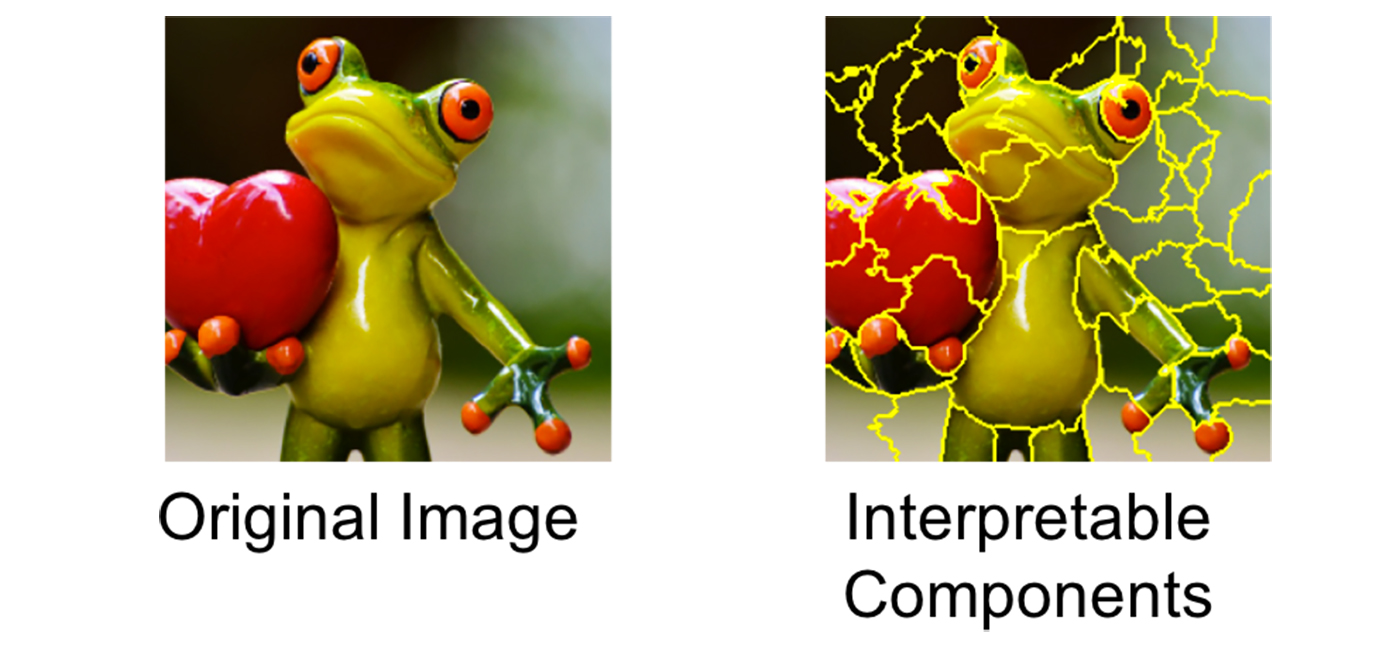
\includegraphics[width=14cm]{chapters/02_methods/images/lime.jpg}
\caption{Superpixels generated for an input image. Superpixels are the features LIME analyzes to }
\end{figure}



\begin{figure}[H]
\centering
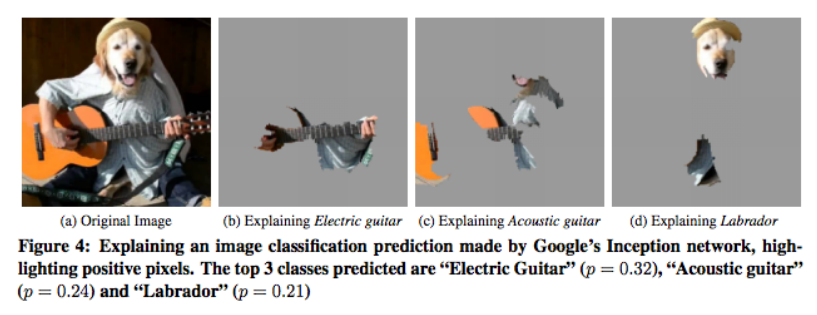
\includegraphics[width=14cm]{chapters/02_methods/images/lime.png}
\caption{Image from original LIME paper explaining three classes}
\end{figure}
